\documentclass{svproc}

\usepackage{graphicx}
\graphicspath{{../experiments/figures/}}
\usepackage{amsmath,amssymb}
\usepackage{booktabs}
\usepackage{url}
\usepackage{hyperref}
\usepackage{placeins}  % \FloatBarrier to keep figures near their text

\begin{document}
\mainmatter

\title{From Episodes to Abstractions: Latent Hierarchical\\Memory in 1,908 AI Conversations}

\titlerunning{Latent Hierarchical Memory in AI Conversations}

\author{Alex Towell \and John Matta}
\authorrunning{A. Towell and J. Matta}

\institute{Southern Illinois University Edwardsville,
Edwardsville, IL, USA\\
\email{\{atowell, jmatta\}@siue.edu}}

\maketitle

% ============================================================================
\begin{abstract}
We investigate whether AI conversation archives---externalized records of
knowledge exploration through dialogue with large language models---contain
hierarchical structure analogous to human semantic memory. From a longitudinal
archive of 1,908 ChatGPT conversations spanning 29 months, we extract semantic
concepts using LLM-based analysis, embed them in a 768-dimensional semantic
space, and apply hierarchical agglomerative clustering to organize them into a
four-level hierarchy: 500 \emph{meta-concepts} $\to$ 50 \emph{themes} $\to$ 8
\emph{knowledge domains}. The concept co-occurrence network is
small-world ($\sigma \approx 6.6$, validated against 100
Erd\H{o}s-R\'{e}nyi random graphs), matching the topology reported for
human semantic memory networks. Meta-concept vocabulary follows Heaps' law
($\beta = 0.320$), with growth dynamics distinguishable from both random
clustering and a bipartite configuration null preserving degree sequences
($p < 0.001$ for both), indicating genuine categorical structure.
The bipartite graph further reveals that 77\% of episodes span multiple
knowledge domains through shared concepts, and that cross-domain concept
sharing is concentrated in specific domain pairs rather than distributed
uniformly.
\keywords{semantic memory, hierarchical clustering, knowledge networks,
complementary learning systems, AI conversations, small-world networks}
\end{abstract}

% ============================================================================
\section{Introduction}
\label{sec:intro}

Over the past three years, millions of users have engaged in sustained dialogue
with large language models (LLMs), producing conversation archives that constitute
an unprecedented record of externalized knowledge exploration~\cite{zhao2024wildchat}.
A single user's ChatGPT history may contain thousands of episodes spanning
programming, mathematics, philosophy, and creative writing---each episode a trace
of a specific learning or problem-solving encounter. Yet these archives are
typically treated as flat, chronological lists, discarding whatever structure might
exist in the knowledge they collectively represent.

We ask: \emph{does hierarchical structure emerge from these conversation archives
when viewed through the lens of cognitive memory theory?}

Complementary Learning Systems (CLS)
theory~\cite{mcclelland1995there,kumaran2016learning} provides a principled
framework. CLS posits two interacting memory systems: a \emph{hippocampal} system
that rapidly encodes individual episodes, and a \emph{neocortical} system that
gradually extracts statistical regularities, forming abstract semantic knowledge.
A prediction of this process is that novel experiences increasingly map to
existing categories rather than creating new ones---a phenomenon measurable
through vocabulary growth dynamics.

Independently, research on human semantic memory networks has established that
conceptual knowledge organizes into \emph{small-world}
networks~\cite{steyvers2005large,siew2019cognitive}: high local clustering with
short global path lengths. Steyvers and Tenenbaum~\cite{steyvers2005large} showed this topology holds
across Roget's Thesaurus, WordNet, and word association
norms~\cite{dedeyne2019small}, with clustering-to-path-length ratios
corresponding to $\sigma$ values of 5.6--15.3 under the later Humphries--Gurney
formulation~\cite{humphries2008network}.

We apply these cognitive frameworks to a longitudinal archive of 1,908 ChatGPT
conversations spanning December 2022 through April 2025. Our approach is
bottom-up: we use an LLM to extract fine-grained semantic concepts from each
episode, embed them in a shared vector space, and allow hierarchical structure
to emerge through geometric clustering. The central contributions are:

\begin{enumerate}
    \item A bipartite episode--concept graph and four-level hierarchy
          (1,908 episodes $\to$ 500 meta-concepts $\to$ 50 themes $\to$
          8 domains) with interpretable knowledge categories at each level;
    \item Sublinear vocabulary growth (Heaps' law $\beta = 0.320$),
          with growth dynamics distinguishable from a random-clustering null
          model ($p < 0.001$), showing that semantic structure creates
          meaningful categorical distinctions;
    \item Small-world topology ($\sigma \approx 6.6$, against 100 Erd\H{o}s-R\'{e}nyi
          random graphs) in the concept co-occurrence network, consistent with
          human semantic memory benchmarks;
    \item Many-to-many episode--concept associations, where 77\% of episodes span
          multiple knowledge domains---structure invisible to partition-based methods;
    \item Size-normalized asymmetric concept sharing between domains, revealing
          genuine semantic isolation punctuated by specific cross-domain dependencies.
\end{enumerate}

% ============================================================================
\section{Related Work}
\label{sec:related}

\paragraph{Complementary Learning Systems.}
CLS theory~\cite{mcclelland1995there,kumaran2016learning} explains how hippocampal
episodic encoding and neocortical consolidation interact. The hippocampal system
rapidly encodes individual experiences with pattern separation, while the
neocortical system gradually extracts statistical regularities through
interleaved replay. A key prediction is that novel experiences increasingly
map to existing semantic categories---a form of vocabulary saturation that
can be measured through growth dynamics like Heaps'
law~\cite{heaps1978information}. Heaps' law ($V(n) = K \cdot n^\beta$)
was originally formulated for natural language vocabulary growth,
where $\beta \approx 0.4$--$0.6$~\cite{lti2009heaps}; lower $\beta$ indicates
stronger consolidation.

\paragraph{Cognitive Network Science.}
Semantic memory networks exhibit small-world
topology~\cite{watts1998collective}---high local clustering with short
global path lengths~\cite{steyvers2005large,siew2019cognitive}.
Collins and Loftus~\cite{collins1975spreading} proposed spreading activation as
the retrieval mechanism; Rosch~\cite{rosch1975cognitive} established
hierarchical categorization. De Deyne et al.~\cite{dedeyne2019small} confirmed
small-world properties across 12,000 cues in a word association network.
The small-world coefficient
$\sigma = (C/C_\text{rand}) / (L/L_\text{rand})$,
as formalized by Humphries and Gurney~\cite{humphries2008network},
compares observed clustering and path lengths to
Erd\H{o}s-R\'{e}nyi random graphs with matched node and edge counts. From the clustering and path length ratios reported by Steyvers and
Tenenbaum~\cite{steyvers2005large}, one can compute $\sigma$ values of
5.6--15.3 across their three semantic networks, supporting their argument
that small-world structure is a universal property of semantic memory.

\paragraph{Topic Modeling and Hierarchical Theme Discovery.}
LDA~\cite{blei2003latent} discovers latent themes from word co-occurrence
statistics; BERTopic~\cite{grootendorst2022bertopic} extends this with
transformer embeddings and hierarchical topic merging. Hierarchical
Dirichlet Processes~\cite{teh2006hierarchical} learn topic hierarchies
nonparametrically. These approaches discover latent themes but do not produce named,
interpretable concept nodes linked to specific episodes in a bipartite graph
that supports downstream network analysis.

\paragraph{LLM-Based Knowledge Extraction.}
Recent work uses LLMs for ontology
construction~\cite{funk2023towards} and knowledge graph
construction~\cite{pan2024unifying}. Graph
RAG~\cite{edge2024graphrag} uses LLM community summarization for
retrieval-augmented generation. These systems extract structured knowledge
from text but focus on downstream retrieval rather than analyzing the
\emph{structure} of the extracted knowledge itself.

\paragraph{Conversation Corpus Analysis.}
Large-scale LLM conversation datasets include
WildChat~\cite{zhao2024wildchat} (1M ChatGPT interactions),
LMSYS-Chat-1M~\cite{zheng2024lmsys} (1M multi-model conversations), and
OpenAssistant~\cite{kopf2023openassistant} (161K crowd-sourced messages).
These corpora support behavioral analysis and model evaluation but do not
examine the semantic structure of individual user archives over time.
Our prior work~\cite{towell2025cognitive} constructed a semantic similarity
network from the same archive using Louvain
partitioning~\cite{fortunato2010community}. The present work differs
fundamentally: extracting explicit concepts produces a bipartite graph
capturing many-to-many associations that partition-based methods cannot
represent.

% ============================================================================
\section{Data and Methods}
\label{sec:methods}

\subsection{Dataset}

The dataset comprises 1,908 ChatGPT conversations from a single user's archive,
spanning December 2022 through April 2025 (29 months), containing 35,411
messages (16,503 user, 18,908 assistant). Conversations range from 2 to 416
messages (median 10, mean 18.6), covering statistical methodology, software
engineering, AI research, R programming, physics, philosophy, and creative
projects across multiple model generations (GPT-3.5 through GPT-4o and o1/o3).
The archive represents a naturalistic record of sustained AI-assisted knowledge
exploration by a single researcher; it is not crowd-sourced or curated for
particular topics.

\subsection{Concept Extraction}

We extract semantic concepts from each episode using Claude Sonnet
3.5 v2\footnote{Model ID: \texttt{claude-3-5-sonnet-20241022}, temperature $= 0$.}
via the Anthropic API. For each episode, the model receives the first
20 messages of the conversation (each capped at 500 characters) and a
structured prompt requesting 3--10 noun-phrase
concepts (2--5 words each) capturing the specific knowledge explored. The
prompt instructs: \emph{``Be specific---use `Metropolis-Hastings algorithm'
rather than `statistics.' Focus on what knowledge is explored, not how the
conversation proceeds.''}

To process all 1,908 conversations efficiently, we deploy 20 parallel
extraction agents, each operating independently on a partition of episodes.
Because agents run in parallel, they cannot share a running vocabulary;
post-hoc deduplication is performed geometrically via hierarchical clustering
(\S\ref{sec:clustering}).

\subsection{Concept Embedding}

Each unique concept is embedded using the
\texttt{nomic-embed-text} model~\cite{nussbaum2024nomic}, which produces
768-dimensional vectors (the native output dimension of its BERT-derived
architecture; this is not a hyperparameter choice). The model was trained
via contrastive learning on diverse text and supports 8,192-token context.
Embeddings are L2-normalized to enable cosine similarity comparisons.

\subsection{Hierarchical Clustering}
\label{sec:clustering}

We apply hierarchical agglomerative clustering (Ward
linkage~\cite{ward1963hierarchical}, Euclidean distance) to the concept embedding
matrix and cut the dendrogram at three heights, producing four levels:

\begin{itemize}
    \item \textbf{Level 0}: 1,908 episodes (individual conversations)
    \item \textbf{Level 1}: 500 meta-concepts (semantic deduplication)
    \item \textbf{Level 2}: 50 themes (broad topic groups)
    \item \textbf{Level 3}: 8 domains (top-level knowledge areas)
\end{itemize}

\noindent The meta-concept level ($k = 500$) groups semantically equivalent
concepts from parallel extraction agents (e.g., ``bootstrap confidence
intervals'' and ``BCa bootstrap confidence intervals''). Cut points are chosen
for interpretability rather than optimality: silhouette analysis shows
monotonically increasing scores for $k \geq 20$ with no distinct peak,
indicating the absence of natural cluster boundaries in the embedding space.
The sensitivity analysis in Table~\ref{tab:sensitivity} confirms that
qualitative findings (sublinear growth, small-world topology) are robust
across $k = 200$--$1{,}000$.

\subsection{Bipartite Graph and Co-occurrence Network}

We construct a bipartite graph $G = (E \cup C, L)$ where $E$ is the set of
1,908 episodes, $C$ is the set of 500 meta-concepts, and $(e, c) \in L$
whenever episode $e$ was assigned at least one raw concept belonging to
meta-concept cluster $c$. This yields 7,153 bipartite edges (mean 3.75
meta-concepts per episode, compared to 3.96 raw concepts per episode). From this bipartite graph, we derive a weighted
co-occurrence network on meta-concepts: two meta-concepts $c_i, c_j \in C$
are linked whenever they co-occur in at least one episode, with edge weight
$w(c_i, c_j) = |\{e \in E : (e, c_i) \in L \wedge (e, c_j) \in L\}|$.

% ============================================================================
\section{Results}
\label{sec:results}

\subsection{Concept Extraction and Deduplication}

Extraction yields 7,555 raw concept mentions (3.96 per episode) mapping to
3,517 unique concepts after case-insensitive deduplication. The raw distribution is
long-tailed: 79.4\% of concepts appear in only one episode. The 500-cluster
meta-concept level consolidates this further: singletons drop to ${<}1\%$,
and the mean frequency rises from 2.1 to 14.3 episodes per meta-concept
(Table~\ref{tab:dedup}, Fig.~\ref{fig:frequency}).

\begin{table}[!htb]
\centering
\caption{Effect of meta-concept deduplication on bipartite graph density.}
\label{tab:dedup}
\begin{tabular}{lrr}
\toprule
Metric & Raw concepts & Meta-concepts \\
\midrule
Unique concepts & 3,517 & 500 \\
Singletons (\%) & 79.4 & $<1$ \\
Mean episodes/concept & 2.1 & 14.3 \\
Episode pairs sharing concepts & 9,304 & 165,000 \\
\bottomrule
\end{tabular}
\end{table}

\begin{figure}[!htb]
\centering
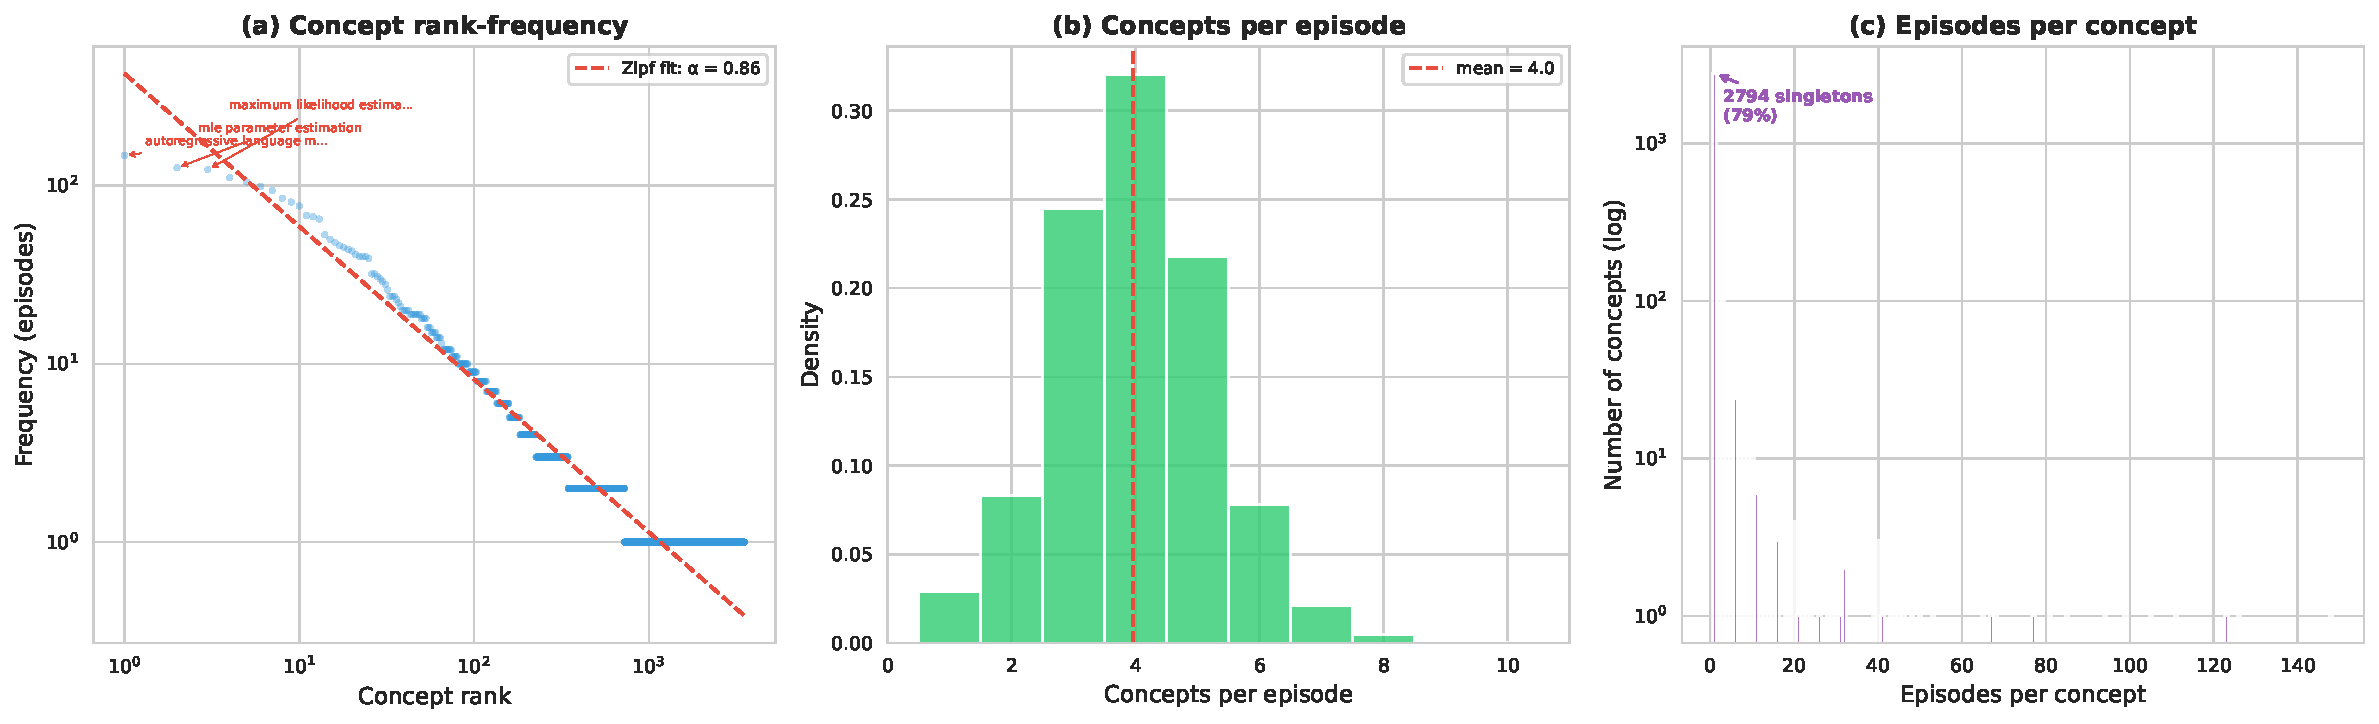
\includegraphics[width=\textwidth]{semantic_frequency_distributions.pdf}
\caption{Concept frequency distributions. \textbf{Left}: Zipf rank-frequency
plot (Zipf exponent $\approx 0.86$). \textbf{Center}: Concepts per episode
(mean 3.96). \textbf{Right}: Episodes per concept showing the long tail
(79\% singletons).}
\label{fig:frequency}
\end{figure}

\subsection{Latent Hierarchy}

Ward linkage at $k = 8$ produces eight interpretable knowledge domains
(Table~\ref{tab:domains}). The bipartite structure allows episodes to span
multiple domains: only 22.5\% are confined to a single domain; 42\% span two,
25\% span three, and 10\% span four or more.
Episodes spanning 3+ domains (35\%) function as cross-domain integration
points---e.g., ``automatic differentiation for MLE in R'' spans Software
Engineering, Statistics, and Mathematics
(Fig.~\ref{fig:cooccurrence}).

\begin{table}[!htb]
\centering
\caption{Eight knowledge domains from Ward linkage clustering.}
\label{tab:domains}
\begin{tabular}{lrp{4.2cm}}
\toprule
Domain & Raw concepts & Representative concepts \\
\midrule
Software Engineering & 1,074 & code refactoring, API design \\
Math \& Optimization & 634 & simulation, Fisher info. \\
Statistical Methods & 510 & MLE, bootstrap, Weibull \\
Philosophy \& AI Theory & 489 & consciousness, complexity \\
ML \& Network Science & 274 & language models, networks \\
DevOps \& Integration & 273 & APIs, hosting, admin \\
AI Safety \& Research & 177 & alignment, evaluation \\
LLM Engineering & 86 & prompts, agents, tools \\
\bottomrule
\end{tabular}
\end{table}

\begin{figure}[!htb]
\centering
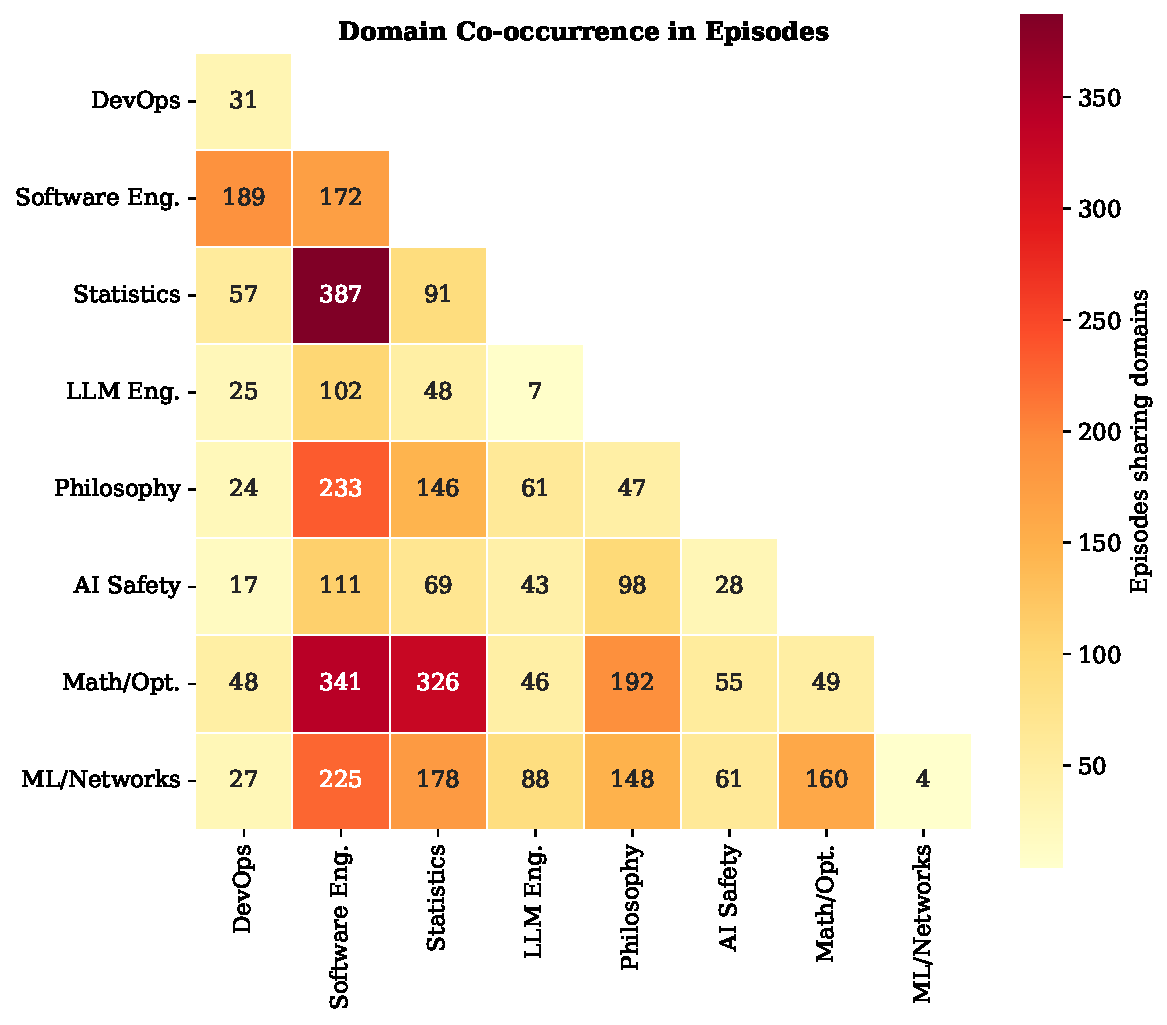
\includegraphics[width=0.85\textwidth]{domain_cooccurrence.pdf}
\caption{Domain co-occurrence heatmap showing how many episodes span
each pair of domains. Software Engineering co-occurs broadly; specialized
pairs (Statistics--Math) show focused affinity.}
\label{fig:cooccurrence}
\end{figure}

\subsection{Vocabulary Growth and Null Model}

Processing episodes in alphabetical order by ID, the meta-concept vocabulary
grows sublinearly following Heaps' law
$V(n) = K \cdot n^\beta$ with $\beta = 0.320$ (Fig.~\ref{fig:heaps}).
Under 100 random episode orderings, $\beta = 0.241 \pm 0.007$, confirming
that sublinear growth is robust to ordering, though the specific $\beta$
value depends on the sequence (alphabetical ordering inflates $\beta$ due to
topical autocorrelation among lexicographically adjacent episode IDs).
The raw concept vocabulary (before clustering) grows nearly linearly
($\beta = 0.931$), confirming that sublinear growth arises from the
clustering step, not the extraction process.

Since clustering at $k = 500$ imposes a vocabulary ceiling that
guarantees sublinear growth regardless of semantic content, we test whether
the observed $\beta$ reflects genuine semantic structure or is purely a
ceiling artifact using two null models of increasing stringency.

\textbf{Null model 1} (cluster permutation): Using the same alphabetical
episode ordering, we randomly permute concept-to-cluster assignments
(preserving cluster sizes) and compute $\beta$ for 1,000 permutations. The
null distribution has $\beta_\text{null} = 0.268 \pm 0.006$, and the
observed $\beta = 0.320$ lies above the entire null distribution
($p < 0.001$).

\textbf{Null model 2} (bipartite configuration): A stricter baseline
randomizes which meta-concepts appear in which episodes while preserving
both marginals (the number of meta-concepts per episode and the number of
episodes per meta-concept) using the Curveball algorithm for uniform
sampling of binary matrices with fixed row and column sums. This null
disentangles temporal exploration dynamics from the bipartite degree
sequence. The result: $\beta_\text{null} = 0.254 \pm 0.007$,
with $p < 0.001$.

Both nulls confirm that the observed growth dynamics
are not artifacts of ceiling effects or degree-sequence constraints.
Semantic clustering produces a \emph{higher} $\beta$ (less sublinear,
closer to linear) than either null: the semantically coherent clusters
create meaningful distinctions, so encountering a genuinely new meta-concept
requires exploring novel intellectual territory rather than merely
encountering new vocabulary.

Clustering sensitivity analysis confirms robustness: $\beta$ increases
monotonically from 0.061 ($k=50$) to 0.467 ($k=1{,}000$), but the
qualitative finding of sublinear growth is stable across $k = 200$--$1{,}000$
(Table~\ref{tab:sensitivity}).

\begin{figure}[!htb]
\centering
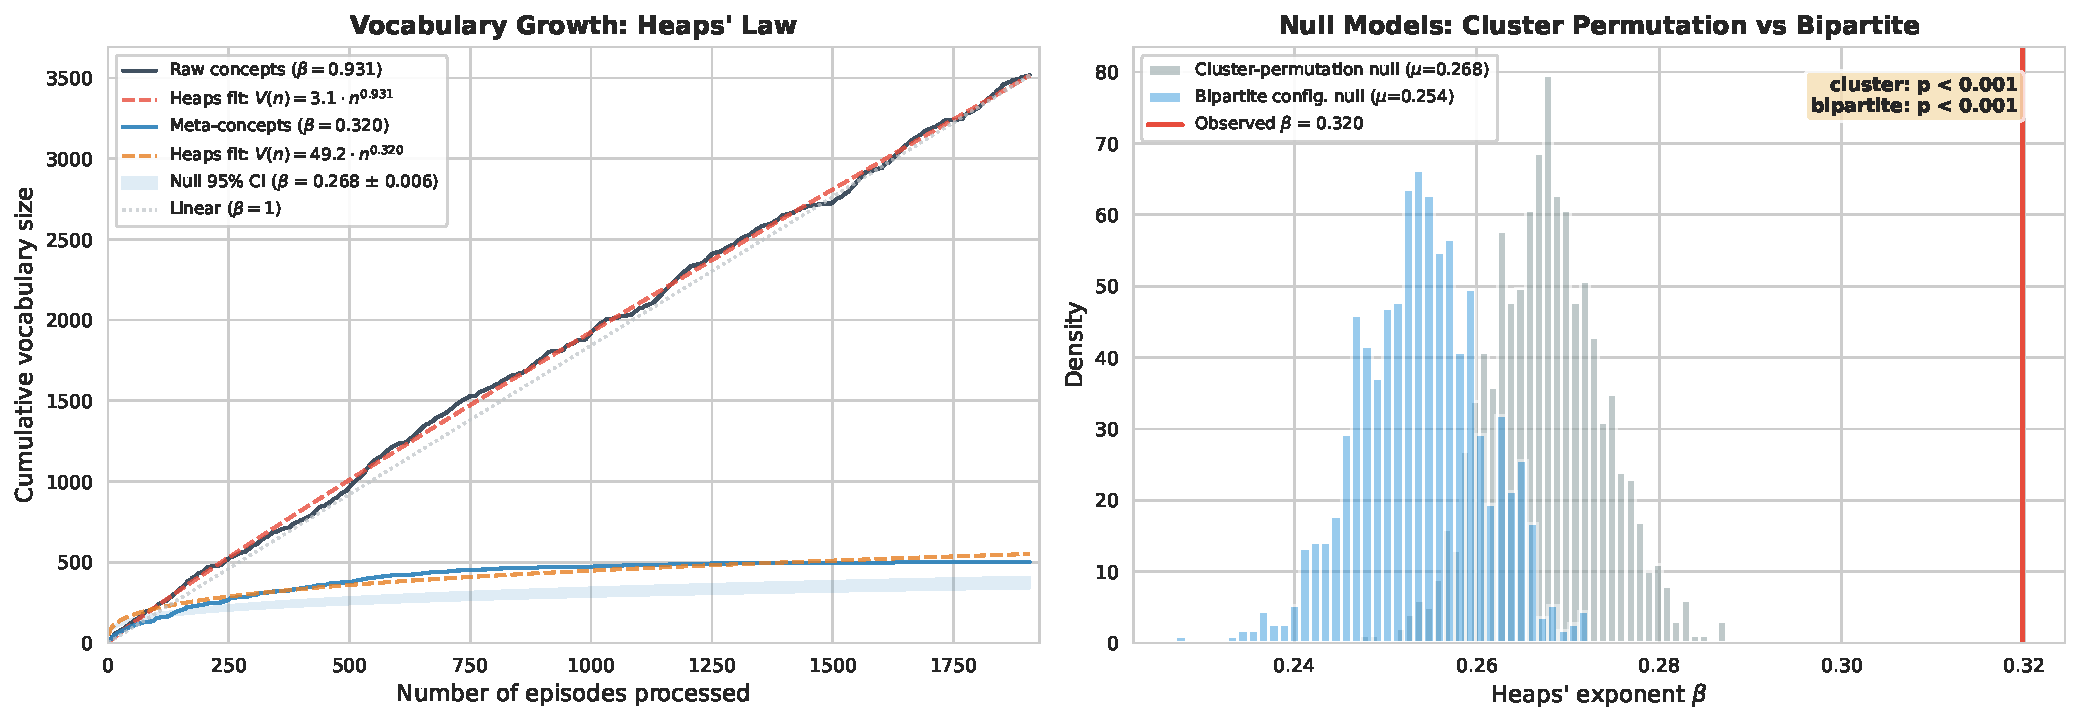
\includegraphics[width=\textwidth]{heaps_law.pdf}
\caption{Vocabulary growth and null model validation.
\textbf{Left}: Cumulative vocabulary following Heaps' law ($\beta = 0.931$ for
raw concepts, $\beta = 0.320$ at the meta-concept level).
\textbf{Right}: Two null model distributions. Gray: cluster-permutation null
($\beta_\text{null} = 0.268$, $p < 0.001$). Blue: bipartite configuration
null preserving both marginals ($\beta_\text{null} = 0.254$, $p < 0.001$).
The observed $\beta = 0.320$ lies entirely above both null distributions.}
\label{fig:heaps}
\end{figure}

\subsection{Small-World Topology}

The meta-concept co-occurrence network (499 of 500 meta-concepts; one
singleton has no co-occurrence edges; 5,935 edges) exhibits
small-world properties (Table~\ref{tab:smallworld}). Following the
Humphries--Gurney formulation~\cite{humphries2008network}, we compare
clustering and path length to 100 Erd\H{o}s-R\'{e}nyi $G(n,m)$ random graphs
with matched node and edge counts. The clustering coefficient is $6.9\times$
higher than random, while the path length is only $1.05\times$ longer, yielding
$\sigma \approx 6.6$. This is comparable to $\sigma$ values derivable from the clustering and
path-length ratios reported for human semantic memory
networks~\cite{steyvers2005large,dedeyne2019small}---Roget's
($\sigma \approx 13$), WordNet ($\sigma \approx 15$), and word associations
($\sigma \approx 5.6$)---though direct comparison is approximate since those
studies used different random graph baselines. Clustering sensitivity
confirms robustness: $\sigma$ ranges from 2.0 ($k=200$) to 12.6 ($k=700$),
remaining above 1 across all tested values of $k$
(Table~\ref{tab:sensitivity}).

\begin{table}[!htb]
\centering
\caption{Small-world analysis of the concept co-occurrence network.
Random graph baselines are means over 100 Erd\H{o}s-R\'{e}nyi $G(n,m)$
graphs.}
\label{tab:smallworld}
\begin{tabular}{lrl}
\toprule
Property & Value & Interpretation \\
\midrule
Nodes & 499 & \\
Edges & 5,935 & \\
Clustering $C$ & 0.329 & \\
$C / C_\text{rand}$ & 6.89 & High local clustering \\
Path length $L$ & 2.37 & \\
$L / L_\text{rand}$ & 1.05 & Short global paths \\
\textbf{Small-world $\sigma$} & \textbf{6.57} & Strongly small-world \\
Mean degree & 23.8 & \\
\bottomrule
\end{tabular}
\end{table}

\begin{table}[!htb]
\centering
\caption{Clustering sensitivity: key metrics across meta-concept granularity $k$.
Both $\beta$ and $\sigma$ vary with $k$ but the qualitative findings (sublinear
growth, small-world topology) are robust across $k = 200$--$1{,}000$.}
\label{tab:sensitivity}
\begin{tabular}{rrrrr}
\toprule
$k$ & Heaps' $\beta$ & $\sigma$ & $C$ & Edges \\
\midrule
50   & 0.061 &  1.1 & 0.830 &    906 \\
100  & 0.103 &  1.4 & 0.652 &  2,286 \\
200  & 0.158 &  2.0 & 0.425 &  4,111 \\
300  & 0.225 &  2.9 & 0.351 &  5,073 \\
\textbf{500} & \textbf{0.320} & \textbf{6.57} & \textbf{0.329} & \textbf{5,935} \\
700  & 0.382 & 12.6 & 0.351 &  6,593 \\
1000 & 0.467 & 25.9 & 0.401 &  7,291 \\
\bottomrule
\end{tabular}
\end{table}

\subsection{Asymmetric Concept Flow}

The bipartite graph enables a directed analysis that the undirected co-occurrence
network cannot capture: for each pair of domains $(A, B)$, we measure the fraction
of $B$'s episodes that contain at least one concept from domain $A$. We call this
fraction the \emph{broadcast reach} of domain $A$---the share of non-$A$ episodes
containing at least one of $A$'s concepts. Conversely, the \emph{porosity} of
domain $A$ is the fraction of $A$'s episodes containing at least one foreign
concept. If concept sharing were symmetric, broadcast reach from $A$ to $B$ would
equal the reverse; in practice, it is asymmetric (Fig.~\ref{fig:flow}).

Software Engineering has the highest broadcast reach (40\% of all non-SE episodes),
penetrating all seven other domains.
However, Software Engineering also contains 30.5\% of all raw concepts (1,074 of
3,517), raising the question of whether its broad reach reflects genuine cross-domain
dependency or a domain size effect. To control for this, we compare observed flow
to a null model that randomly reassigns concept-domain labels (preserving domain
sizes, 100 permutations). The ob\-served/ex\-pected ratios fall below 1.0 for most
domain pairs (mean $= 0.61$), confirming that the eight domains capture genuine
semantic boundaries: concepts cluster within domains more tightly than expected
under random concept-domain assignment.

Within this overall isolation, specific domain pairs show elevated sharing
relative to the null. LLM Engineering $\to$ ML \& Network Science has an
observed/expected ratio of 2.67, and LLM Engineering $\to$ AI Safety reaches
1.27. ML \& Network Science has the highest porosity (30\% of its episodes
contain foreign concepts), functioning as an
interdisciplinary junction where concepts from multiple domains converge.

\begin{figure}[!htb]
\centering
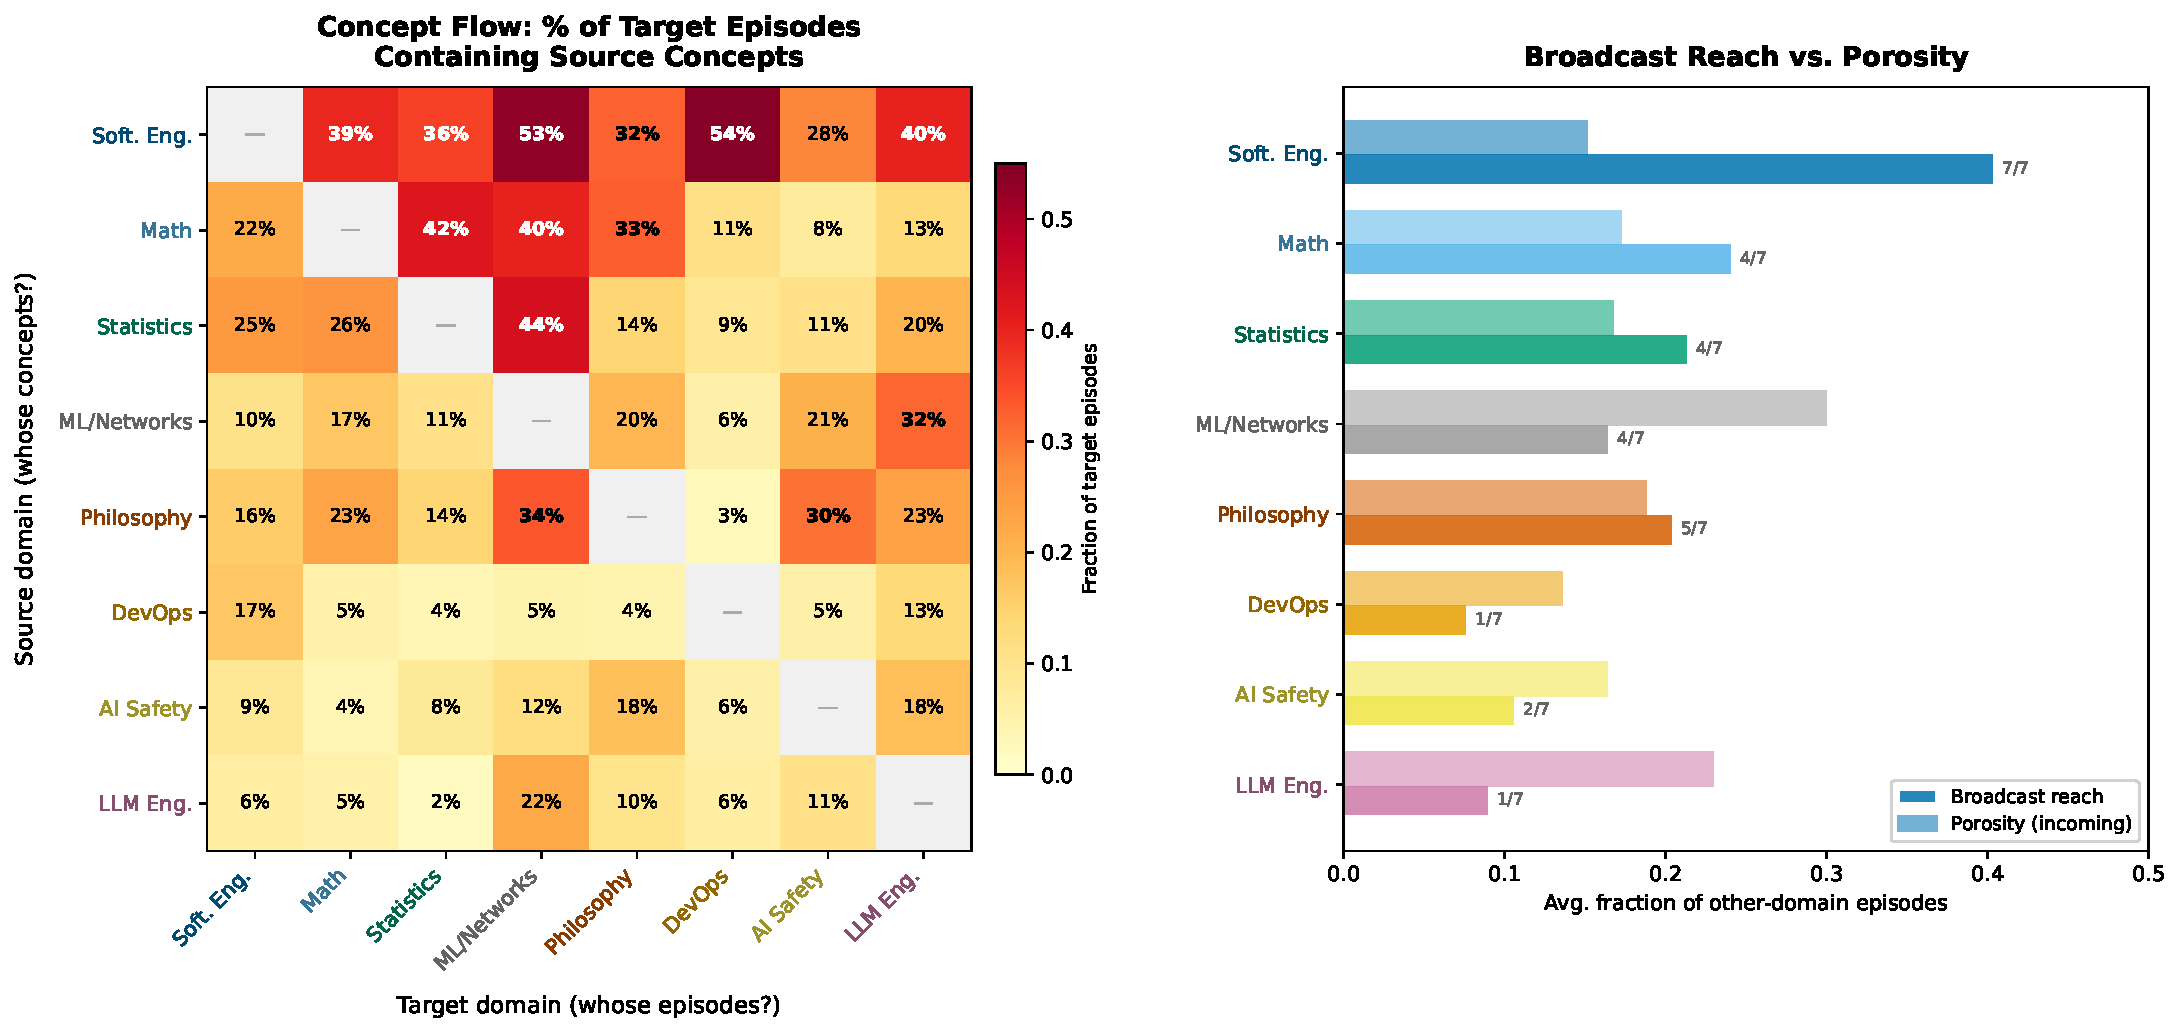
\includegraphics[width=\textwidth]{domain_flow.pdf}
\caption{Asymmetric concept flow between domains. \textbf{Left}: Flow matrix
showing the fraction of target-domain episodes (columns) containing
source-domain concepts (rows). The matrix is asymmetric: Software Engineering
exports broadly (top row), while ML \& Network Science absorbs from all domains
(column~4). \textbf{Right}: Broadcast reach (fraction of foreign episodes
containing a domain's concepts) versus porosity (fraction of a domain's
episodes containing foreign concepts). Numbers indicate reach breadth
(domains penetrated above 15\%).}
\label{fig:flow}
\end{figure}

\subsection{Bipartite Network Visualization}

Figure~\ref{fig:knowledge_map} visualizes the full bipartite structure as a
radial layout: meta-concepts occupy an inner ring, episodes an outer ring, both
grouped by domain sector. Bipartite edges connect episodes to their constituent
meta-concepts, while co-occurrence edges link concepts that share episodes.
The visualization makes the asymmetric flow visible: Software Engineering
episodes (lower right) send concept links into every sector, while Philosophy
episodes (lower left) connect almost exclusively to their own domain's concepts.

\begin{figure}[!htb]
\centering
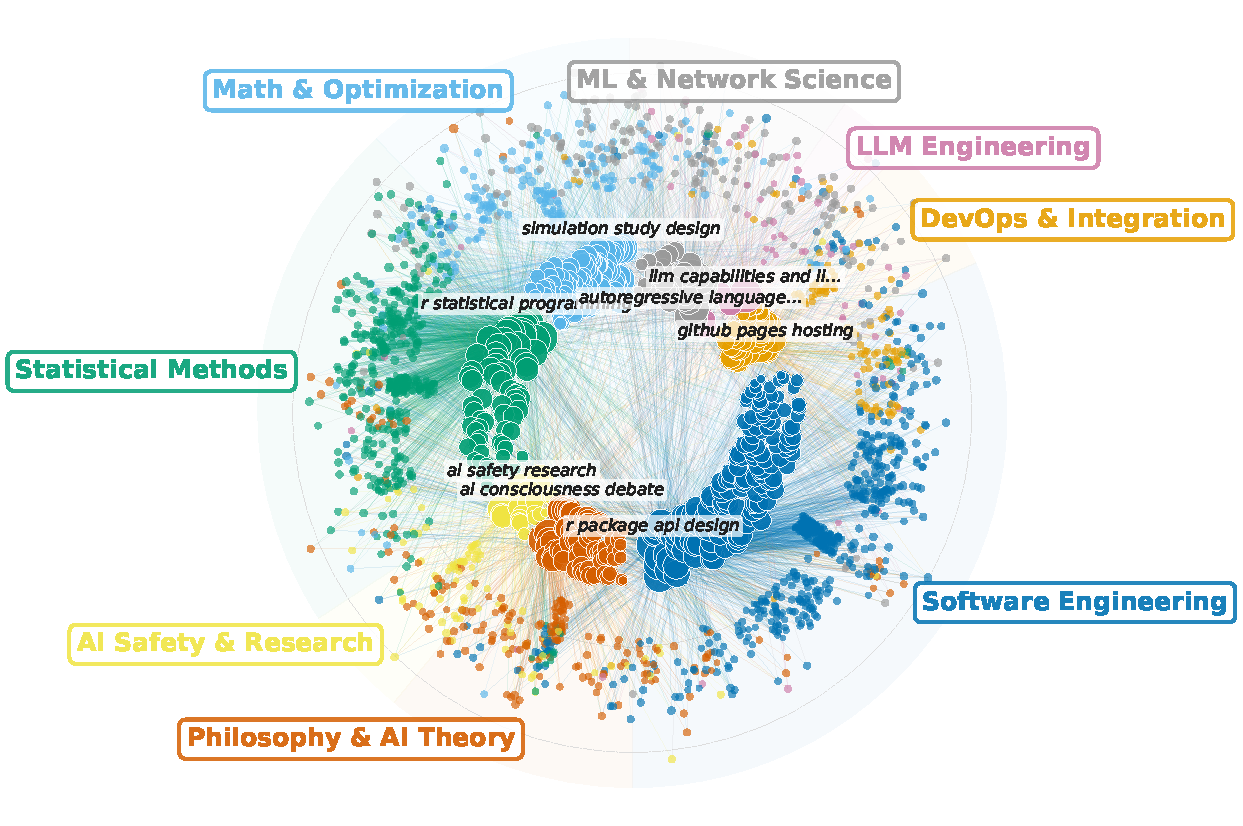
\includegraphics[width=\textwidth]{knowledge_map_bipartite.pdf}
\caption{Bipartite knowledge map. Inner ring: 499 meta-concepts (colored and
sized by domain and frequency). Outer ring: 1,908 episodes (colored by primary
domain). Radial lines show episode--concept associations (filtered to
meta-concepts appearing in $\geq 8$ episodes); gray lines show concept
co-occurrence ($\geq 4$ shared episodes). Sector size is proportional to
episode count. Cross-sector bipartite edges reveal the directed concept flow:
foundational domains export concepts broadly, while applied domains absorb.}
\label{fig:knowledge_map}
\end{figure}

Figure~\ref{fig:bridge} provides a complementary zoom-in view: two specific
episodes from different domains---``AI Language Models Compared'' (Statistical
Methods) and ``Language Models and Computation'' (Philosophy \& AI
Theory)---share five meta-concepts spanning four knowledge domains. These
episodes approach the same intellectual territory (the nature of language model
prediction) from fundamentally different disciplinary angles, yet the bipartite
graph reveals their deep connection through shared concepts like Solomonoff
induction, Kolmogorov complexity, and autoregressive language models. A
partition-based method~\cite{fortunato2010community} would assign these episodes
to separate communities; the bipartite concept hierarchy captures their
relationship explicitly.

\begin{figure}[!htb]
\centering
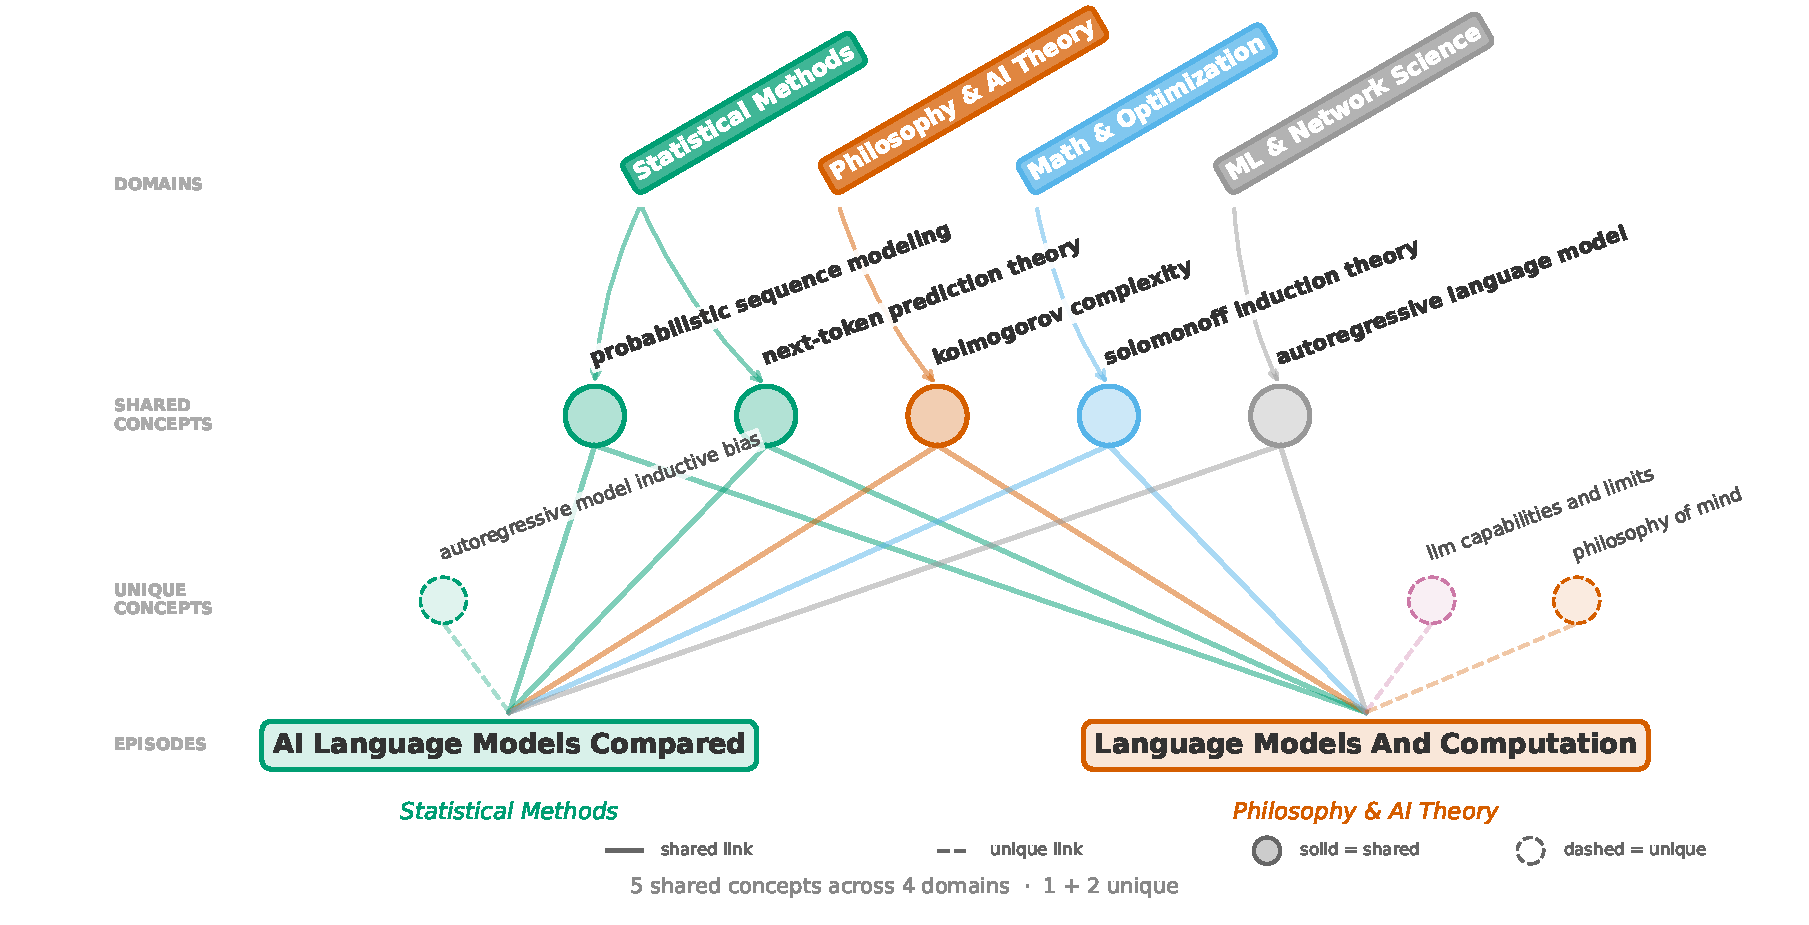
\includegraphics[width=\textwidth]{zoom_in_bridge.pdf}
\caption{Zoom-in: two episodes from different domains connected through shared
concepts. ``AI Language Models Compared'' (Statistical Methods) and ``Language
Models and Computation'' (Philosophy \& AI Theory) share 5 meta-concepts
spanning 4 domains (top row). Solid circles and lines show shared concepts;
dashed circles show concepts unique to each episode. Each episode also has
unique concepts reflecting its disciplinary focus: inductive bias (Statistics)
vs.\ philosophy of mind and LLM capabilities (Philosophy/LLM Engineering).}
\label{fig:bridge}
\end{figure}

\FloatBarrier
% ============================================================================
\section{Discussion}
\label{sec:discussion}

\paragraph{Vocabulary Growth and Semantic Structure.}
The meta-concept vocabulary grows sublinearly ($\beta = 0.320$), but since
clustering at fixed $k = 500$ guarantees sublinear growth regardless of
content, the absolute $\beta$ value is not itself evidence of consolidation.
Two null model comparisons reveal a more nuanced finding: semantic clustering
produces \emph{higher} $\beta$ (less sublinear) than both random cluster
assignment ($\beta_\text{null} = 0.268$, $p < 0.001$) and a stricter
bipartite configuration null that preserves both episode and meta-concept
degree sequences ($\beta_\text{null} = 0.254$, $p < 0.001$). The second
null, which randomizes meta-concept co-occurrence across episodes while
preserving marginals, confirms that the observed growth dynamics reflect
genuine temporal exploration structure, not merely the bipartite degree
sequence. Under either null, conceptually unrelated items share clusters
by chance, so any new episode is likely to fall into an existing cluster
through accidental overlap; under semantic clustering, clusters are internally
coherent and only genuinely related episodes share a meta-concept.
CLS theory would predict that meaningful categories \emph{facilitate}
consolidation (lower $\beta$), but we observe the opposite: semantically
coherent categories \emph{resist} consolidation. This suggests that the
archive's categorical structure maintains discriminable knowledge
representations---a property consistent with the role of semantic memory in
preserving distinctions, even if it does not follow the consolidation-efficiency
prediction of CLS.

\paragraph{Small-World Topology and Comparison with Human Memory Networks.}
The small-world coefficient $\sigma \approx 6.6$, validated against 100
Erd\H{o}s-R\'{e}nyi random graphs~\cite{humphries2008network}, falls within the
range reported for human semantic memory networks
($\sigma \approx 5$--$15$)~\cite{steyvers2005large}. This convergence
provides a direct quantitative comparison: the AI conversation archive
exhibits the same balance of local coherence and global accessibility
observed in human word association and category fluency networks.
While we do not claim
conversation archives \emph{are} semantic memory, this structural similarity
suggests they function as an externalized analog: concepts connected through
co-occurrence in knowledge episodes, exhibiting the same balance of local
coherence and global accessibility. The sensitivity analysis
(Table~\ref{tab:sensitivity}) shows $\sigma > 1$ is robust across
$k = 100$--$1{,}000$, with the qualitative finding independent of the
specific clustering granularity.

\paragraph{Many-to-Many Associations and Cross-Domain Flow.}
The bipartite graph captures knowledge polysemy: 77\% of episodes span multiple
domains, with 35\% spanning three or more. Partition-based
methods~\cite{fortunato2010community} cannot represent this multiplicity.
The bipartite structure also reveals asymmetric concept flow between domains.
After normalizing for domain size, most cross-domain flow is \emph{below}
what random concept-domain assignment would predict (mean observed/expected
$= 0.61$), confirming that the domains represent genuine semantic clusters
rather than arbitrary partitions. A few specific pairs show elevated flow
(LLM Engineering $\to$ ML \& Network Science at $2.67\times$ expected),
suggesting targeted conceptual dependencies. For downstream applications
like Graph RAG~\cite{edge2024graphrag}, the bipartite structure and domain
hierarchy could enable concept-level indexing and retrieval.

\paragraph{Limitations.}
This is a single-user case study; different users would produce different
concept sets and different hierarchies. We frame this work as a
\emph{proof-of-concept} that motivates, rather than establishes,
generalization. Validating whether sublinear growth and small-world topology
are preserved across users requires replication on multi-user corpora such
as WildChat~\cite{zhao2024wildchat} or LMSYS-Chat-1M~\cite{zheng2024lmsys}.
Hierarchy cut points ($k = 500, 50, 8$) are chosen for interpretability,
not discovered; the silhouette analysis shows generally increasing scores
with $k$ (monotonic for $k \geq 20$, with no distinct peak),
indicating no natural cluster boundaries. Automated thresholding methods
(e.g., gap statistic, stability-based selection) could reduce this
subjectivity. Concept extraction depends on the specific LLM and prompt used;
alternative models or prompts would produce different concept sets, though
the downstream structural properties (small-world, Heaps' law) may be more
robust than the specific concept vocabulary. Despite these limitations, the
convergence with human semantic memory benchmarks across multiple
independent metrics (small-world topology, vocabulary growth dynamics,
cross-domain integration patterns) suggests that the structural properties
may reflect general features of categorical knowledge systems rather than
idiosyncrasies of this particular archive.

\FloatBarrier
% ============================================================================
\section{Conclusion}

We have shown that 1,908 AI conversations contain latent hierarchical structure.
LLM-extracted concepts organize into a four-level hierarchy with
interpretable domains, sublinear vocabulary growth validated against two null
models of increasing stringency (cluster permutation and bipartite
configuration, both $p < 0.001$),
and small-world topology ($\sigma \approx 6.6$, against 100 random graphs)
matching human semantic memory benchmarks. The bipartite
structure captures cross-domain integration that partition-based methods
miss, while size-normalized flow analysis reveals genuine semantic isolation
between domains punctuated by specific cross-domain conceptual dependencies.
These results, presented as a single-user case study,
position AI conversation archives as structured knowledge artifacts whose
organization exhibits structural parallels---particularly small-world
topology---with human semantic memory networks.

\paragraph{Data and Code Availability.}
\begin{sloppypar}
Code for the analysis pipeline is available at
\url{https://github.com/queelius/chatgpt-complex-net}
(DOI: 10.5281/zenodo.15314235).
\end{sloppypar}

% ============================================================================
\bibliographystyle{splncs04}
\bibliography{refs}

\end{document}
